\documentclass[english,a4paper,twoside]{report}

\usepackage{design}

\acrodef{RU}{Reykjavík University}
\acrodef{CADIA}{Center for Analysis \& Design of Intelligent Agents}
\acrodef{RSS}{Rich Site Summary}

% Document meta data.
%FIXME: better title & remove draft suffix
\title{Ambient Earth\\
       {\Large \emph{Design Document --- 1$^{\text{st}}$ draft\/}}}
\author{Christian Luijten\\\url{christian06@ru.is}}
\date{\today}
\institution{
 CADIA group \\
 School of Science and Engineering \\
 Reykjavík University, Reykjavík \\[1em]
 \emph{Under supervision of:\/} \\
 Kristinn R. Thórisson, Ph.D. (Reykjavík University) \\
 dr.ir. Huub van de Wetering (Eindhoven University of Technology) \\
}

\begin{document}

\maketitle

% \abstract{
  % Ambient Earth is a software system for analysis of Internet activity. This
  % document describes the design of the system.
 % }

\tableofcontents

\chapter{Introduction}

This document describes the design of the \AmbE\ project. The ambitional goal
of this project is to give an ambient view on the activity on the whole
world-wide web. In practice, it shows the activity on for instance a forum or
larger weblog system.

The name of the system is \Amber{}.

The design of the project will follow the Constructionist Design Methodology
for Interactive Intelligences\cite{CDM}. First, a few usage scenarios are given
in Chapter~\ref{cpt:scenarios}. These scenarios result in the requirements
which are listed in Chapter~\ref{cpt:requirements}. Using the requirements, an
architecture is written up in Chapter~\ref{cpt:architecture}.

Please note that in this document some basic knowledge of the terminology of
Psyclone framework is assumed. For more information about Psyclone, refer to
the documentation at \url{http://www.cmlabs.com/psyclone/manual/}.


\chapter{\label{cpt:scenarios}Usage scenarios}

\section{A story is posted to a weblog}

When a story is posted on a weblog, it will show up in its RSS feed (this
happens of course outside of our responsibility). If \Amber\ is monitoring this
particular weblog, it will retrieve the story and analyze it. The story is then
displayed on a screen using the results of the analysis.

To get a more concrete idea, suppose \Amber\ is monitoring various A.I. related
weblogs and we would like to find out what they are mainly writing about. We
configure the analysis component in such a way that it can decide whether a
certain subject is dealt with in a story, thereby creating a profile for every
story. Stories with similar subjects will then show up close to eachother in
the display, stories with orthogonal subjects will be very far apart.

The result is an image with various ``clouds'' of in some way related stories.

\section{A discussion is held on a web forum}

Discussions on web forums can get lengthy and the main subject can change
multiple times during their lives. To get an idea what subjects the whole
discussion has been about, \Amber\ can show a cloud map of (part of) the
discussion. It could even show an animation to show how the discussion
developed over time.

Using the animated view of the discussion development, a new participant in the
discussion can decide upon whether bringing up an old discussion point is a
good idea or not. It is also a way to locate a certain subject within a long
list of replies.



\chapter{\label{cpt:requirements}Requirements}

There are various kinds of requirements to be identified. A distinction can be
made between functional and extra-functional (or non-functional) requirements.

\section{Extra-functional requirements}

\begin{enumerate}
  \item The system must make use of the Psyclone framework for communication.
  \item The system will be implemented in the Java programming language.
  \item The display module with the Java Applet must be able to run on any
        machine with a properly installed Java Virtual Machine (i.e. not only
        on the machine running the rest of the system).
  \item It must be possible to add modules with similar functionality to
        operate in parallel with modules already there. For example when the
        Java Applet is running, it should also be possible to have the full
        screen module running at the same time. 
\end{enumerate}

\section{Functional requirements}

These requirements describe which \emph{inputs}, \emph{outputs}, \emph{storage}
and \emph{computations} exist in the system and how they are \emph{timed and
synchronized}. Finally, since this is a very important part of the project,
there are two separate sections on \emph{story analysis} and
\emph{visualization} requirements.

\subsection{Inputs}

\begin{enumerate}
  \item The system must be configurable to specify which sources will be
        monitored.
  \item The system will use the configuration to get information from the
        internet from the specified sources.
  \item Configuration of the system goes via Psyclone using module parameters.
  \item The display may have a set of controls to navigate through the history
        of a feed.
  \item Parts of the system must accept triggers from Psyclone whiteboards.
  \item Sources must be \ac{RSS} feeds. The system should however be prepared
        to support other source types as well (i.e. it should be easily
        expandable).
  \item The Applet display is non-interactive (no input).
\end{enumerate}

\subsection{Outputs}

\begin{enumerate}
  \item There is an output module which is to be used within a website,
        i.e. a Java Applet.
  \item There is an output module which runs standalone and in full screen
        and displays more information than the Applet can.
\end{enumerate}

\subsection{Storage}

\begin{enumerate}
  \item The system on itself does not store anything.
\end{enumerate}

\subsection{Computations}

\begin{enumerate}
  \item The system must decide of a delivered story what its subject(s) is/are.
  \item The system may put weights on the subjects instead of a boolean value.
\end{enumerate}

\subsection{Timing and synchronization}

Synchronization between modules is handled by Psyclone, so no requirements need
to be added to the system itself.

\subsection{Story analysis}

\begin{enumerate}
  \item When stories come in, they are analysed by analysis modules.
  \item Every module adds some meta-information to the story depending on the
        module analysis.
\end{enumerate}

\subsection{Visualization}

The following requirements are common for both the applet and the standalone
viewer.

\begin{enumerate}
  \item A story is represented as a dot.
  \item In the center of the display is Earth (with picture?).
  \item Dots are launched into orbit around Earth.
  \item The orbits follow Kepler's laws of planetary motion.
  \item The launch velocity is dependent on how ``big'' the story is (like from
        an important author or if it has many references) at the time of
        writing, but is always smaller than the escape velocity.
  \item Stories get velocity boosts by getting replies/comments or
        references (``trackbacks'') in order to keep them around longer.
  \item Stories which don't get reactions will just orbit Earth for a while and
        eventually fall back down \mbox{(i.e. launch velocity $<$ escape
        velocity)}.
  \item Only the meta-information added to the stories by the Sieve modules is
        used to determine launch variables.
  \item There are some small, heavy bodies in geostationary orbit around Earth
        representing values of an enumeration of meta-information (for instance
        story subjects). They attract the stories depending on how much they
        match the story's subject. It is possible for a story to get into orbit
        with such a heavy body if it is really strongly connected to the
        subject.
\end{enumerate}

There will be two different views, a static and a dynamic one. Which one is
used depends on the application. To get an idea of the activity at a certain
moment in time, the static view is used. For a ``real-time'' view of internet
activity, the dynamic view can be used.

The term ``static'' doesn't mean the image is standing still, it will behave
exactly the same as the dynamic view. However, some physical laws don't apply
or are differently calibrated in order to give a constant image. In other
words, while in dynamic view stories can appear and disappear, in the static
view the stories are a given constant.

\subsubsection{Differences between Applet and Standalone viewer}

\begin{enumerate}
  \item The applet display will in practice be considerably smaller than the
        standalone viewer. Therefore, the applet is less detailed and some
        physical laws might need to be bend a bit.
\end{enumerate}



\chapter{\label{cpt:architecture}Architecture}

The architecture of \Amber\ is defined in terms of modules and the messages
they use to communicate. A global architecture is depicted in
Figure~\ref{fig:global-architecture}.

In the Section~\ref{sct:modules} the modules are described in detail and in
Section~\ref{sct:messages} the messages connecting them are defined. The data
types used in the system are described in Section~\ref{sct:types}.

\begin{figure}
    \centering
    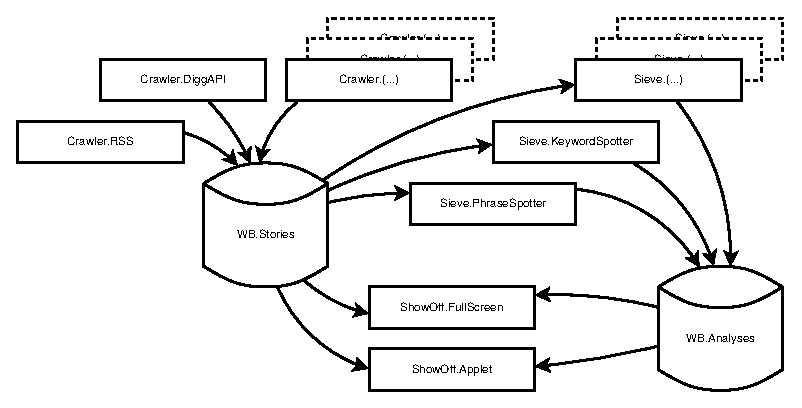
\includegraphics{image/global-architecture}
    \caption{\label{fig:global-architecture}Global \Amber\ architecture, the names are Psyclone module names}
\end{figure}

\section{\label{sct:modules}Modules}

A complete \Amber\ system will comprise at least three modules running at the
same time; there is a Crawler module, an analysis module called Sieve and a
display called ShowOff. The modules are separate executables with their own
life-cycles and resources. Since TCP/IP is used, the executables don't need to
be on the same machine to communicate.

Every module has a specified interface through which communication with
Psyclone is handled.

\subsection{Crawler modules}

When the Crawler is started, it will create one of the available handlers
(depending on what is specified on the command line or what is set as default
during build time). 

It also creates an AirBrush instance to communicate with Psyclone via
Java\-Open\-AIR. The module name announced to Psyclone is `Crawler.' plus the
name of the handler, so `Crawler.RSS' in case of the RSS handler.

After connecting with Psyclone, the handler can get its parameters stored in
the psySpec file and go to work. It will post stories with type `Story'  on the
whiteboard `WB.Stories'.

\subsubsection{RSS}

The RSS crawler module will be fairly straightforward. It fetches the RSS feed
from a set URL and produces a Story message for every new item that appears.
The contents of the Story message is specified in Section~\ref{sct:messages}.

Although the module is called RSS, it can handle Atom feeds, which is also
quite a popular format.

\begin{module}{Crawler.RSS}
  \trigger{Feed.*}{WB.Control}
  \post{Story}{WB.Stories}
\end{module}

\subsubsection{DiggAPI}

Digg is a website which lets users submit stories found on the web. Other users
then moderate the submissions either by `digging' or `burying' a story. A story
with a lot of `diggs' is a popular one. The nice thing about Digg is that it
actually does a lot of preprocessing work for the \Amber\ system.

Digg
announced\footnote{\url{http://diggtheblog.blogspot.com/2006/07/digg-labs-launches-alpha.html}}
that they will publish a public API within the next months. If time allows, a
DiggAPI module is created.

\begin{module}{Crawler.DiggAPI}
    \post{Story}{WB.Stories}
\end{module}

% \subsubsection{BloggerDataAPI}
% 
% One of the larger weblog hosters is Google with their Blogger service. There
% is an API available to get information from it.
% 
% \begin{module}{Crawler.BloggerDataAPI}
%   \post{Story}{WB.Stories}
% \end{module}


\subsection{Sieve modules}

All analysis modules, or sieves, will get a trigger from a new story on the
whiteboard WB.Stories. They analyse it and if it can say anything about the
story, an Analysis message is sent to the whiteboard WB.Analyses containing its
judgement on the story.

The contents of this message is specified in Section~\ref{sct:messages}.

Analysis modules may take any time they like to come to a verdict, but it is
possible that a story has already disappeared from the visualization if the
response is very late.

Since all modules regardless of their functionality employ the same external
behaviour, the Psyclone specification is the same for every one of them.

\begin{module}{Sieve.???}
    \trigger{Story}{WB.Stories}
    \post{Analysis}{WB.Analyses}
\end{module}

\subsection{ShowOff modules}

The ShowOff modules are visualizers which combine the crawled stories from the
Crawler with the analyses from the Sieve modules.

\begin{module}{ShowOff.???}
    \trigger{Story}{WB.Stories}
    \trigger{Analysis}{WB.Analyses}
\end{module}

\subsubsection{Full screen}

The full screen application will display a lot of information and is there to
be looked - not glanced - at. It should be possible to let it do its job
autonomously, just showing a pretty picture, or to be interactive.

\subsubsection{Ambient applet}

The ambient applet will display a very easy to understand image (a glance at it
should be enough) of the status of the page it is on. I.e. if the page is a
weblog, it should display subject information on that weblog, if it is on the
page of a thread of a forum, it displays the flow of the discussion.



\section{\label{sct:messages}Messages}

FIXME: Add life-cycle model of amber.Story.


\subsection{Between Crawler and Sieve}


\subsection{Between Sieve and ShowOff}




\section{\label{sct:types}Data types}

\subsection{Story}

The story type holds the text of an entry, plus meta-data. It is a shared type
between all three modules and it is also exported to the Psyclone whiteboards.

% \begin{type}
  % 
% \end{type}




\chapter{Detailed design}

In this chapter, every single class is described in terms of public interface
and functionality. Because of the fairly dynamic character of this project --
new ideas come and go -- this chapter will not be finished until the end of the
project and will probably change regularly.

\section{Files and directories}

All source code will be in the directory \texttt{src/}. All classes are in the
package \texttt{amber} or in a subpackage thereof. The Psyclone specification
file \texttt{psySpec.xml} is found in \texttt{data/}. External libraries that
are redistributed with \Amber\ are in \texttt{lib/}. The source of this
document, the traineeship report and the website are located in
\texttt{documentation/}.

The application is built using Apache
Ant\footnote{\url{http://ant.apache.org/}} and it can be imported into
Eclipse\footnote{\url{http://www.eclipse.org/}}. It requires Java SDK version
1.5 or greater.

\subsection{Objects in the amber package}

The classes in the main package are launchers for the three different modules
and abstract classes for the main objects of these modules. Basically it works
like this; if the Crawler class is started it creates a CrawlerObject and
starts it.

\classname{Crawler}

\begin{classmetadata}
  \function{The Crawler object makes launching a crawler easy and uniform for
      all crawler types.}
\end{classmetadata}

\begin{interface}
  \init{Crawler}{}
    {Creates an instance of Crawler. Also creates a CrawlerObject and the
      connection to Psyclone.}
  \method{\static\ \void}{main}{String\[\] args}
    {Method executed upon launch of the Crawler.}
  \method{\void}{start}{}
    {Starts the Crawler.}
  \method{\void}{stop}{}
    {Stops the Crawler.}
\end{interface}



\abstractclassname{CrawlerObject}

\begin{classmetadata}
  \function{The CrawlerObject class provides a uniform interface for crawler
      applications.}
  \implements{AirBrushCallable, ModuleInterface}
\end{classmetadata}



\classname{ShowOff}

\begin{classmetadata}
  \function{The ShowOff object makes launching a visualization module easy and
      uniform for all visualizer types.}
\end{classmetadata}

% \begin{interface}
% \end{interface}


\abstractclassname{ShowOffObject}

\begin{classmetadata}
  \function{The ShowOffObject class provides a uniform interface for visualization
      applications.}
  \implements{AirBrushCallable, ModuleInterface}
\end{classmetadata}

\begin{interface}
  \method{\void}{setStoryQueue}{\mbox{Queue$\langle$Story$\rangle$} q}
    {Sets the queue of incoming stories. ShowOff will handle communication with
      the Psyclone whiteboard and puts stories in the queue.}
\end{interface}



\classname{Sieve}

\begin{classmetadata}
  \function{The Sieve object makes launching a analysis module easy and uniform
      for all analyser types.}
\end{classmetadata}

% \begin{interface}
% \end{interface}



\abstractclassname{SieveObject}

\begin{classmetadata}
  \function{The SieveObject class provides a uniform interface for analysis
      applications.}
  \implements{AirBrushCallable, ModuleInterface}
\end{classmetadata}

% \begin{interface}
% \end{interface}



\section{Objects in the amber.common package}

\classname{AirBrush}

\begin{classmetadata}
  \function{Ease communication with Psyclone through JavaOpenAIR.}
\end{classmetadata}

\begin{interface}
  \init{AirBrush}{String moduleName, String hostName, int port}
    {Initializes a connection with Psyclone on \emph{hostName:port} for module
      \emph{moduleName}.}
  \method{\void}{setCallbackObject}{AirBrush\-Callable}
    {Sets the callback object to be used for calls from AirBrush.}
\end{interface}



\interfacename{AirBrushCallable}

\begin{interface}
  \method{\void}{airBrushCallBack}{com.cmlabs.air.Message msg}
    {Used as callback function for the AirBrush.}
\end{interface}



\interfacename{ModuleInterface}

\begin{interface}
  \method{\void}{start}{}
    {Start the module.}
  \method{\void}{stop}{}
    {Stop the module.}
\end{interface}



\classname{Story}

\begin{classmetadata}
  \function{Storage of Story data.}
  \data{Story has a Map$\langle$String, Object$\rangle$ field where it stores
    all data. It also holds a value with the number of analyses left until it
    is considered enough to be visualized. Instead of thrown back on the
    whiteboard with raw stories, it should then go the the processed stories.}
\end{classmetadata}

\begin{interface}
  \method{\static\ \void}{createFromYAML}{String yaml}
    {Creates a Story object, and initializes it from the \emph{yaml} argument
      (see fromYAML method).}
  \method{\void}{setAuthor}{String author}{Sets the author of the story.}
  \method{String}{getAuthor}{}{Gets the author of the story.}
  \method{\void}{setCreationTime}{Date time}{Set the creation time of the story}
  \method{Date}{getCreationTime}{}{Get the creation time of the story.}
  \method{\void}{setContent}{String text}{Set the content of the story.}
  \method{String}{getContent}{}{Get the content of the story.}
  \method{\void}{setValue}{String k, Object v}
    {Store an arbitrary object v under keyword k.}
  \method{Object}{getValue}{String k}
    {Gets the object stored under keyword k.}
  \method{Boolean}{lockForAnalysis}{}
    {Request a lock on the story for analysis. Returns true when given, assumes
      niceness of the analysis modules.}
  \method{\void}{unlock}{}
    {Removes the lock. Again, assumes niceness of the analysis modules.}
  \method{Boolean}{isAnalysisDone}{}
    {Returns true when the story finds it is analysed enough and doesn't need
      another run.}
  \method{\void}{fromYAML}{String yaml}
    {Parses a \ac{YAML} string (e.g. coming from Psyclone) to the contents of the
      object (overwrites values currently stored!). Note, together with toYAML,
      this is the identity function: story.fromYAML(story.toYAML()) = story.}
  \method{String}{toYAML}{}
    {Converts the contents of the object to a \ac{YAML} string to be sent via
      Psyclone.}
\end{interface}



\section{Objects in the amber.crawler package}



\classname{RSS}

\begin{classmetadata}
  \extends{CrawlerObject}
  \implements{AirBrushCallable}
  \processing{An RSS object will accept messages to set its feed source, i.e.
      the feed it should crawl. A message of type `Feed.RSS' or `Feed.Atom'
      will set the source to that URL, whereas a message of type `Feed.OMPL'
      will result RSS to parse this and set all URLs in the \ac{OPML} document
      as source URL.

      It will only post messages of the type `Story' as they are described in
      Section~\ref{sct:messages:story}. No other messages are sent.}
\end{classmetadata}

\begin{interface}
  \init{RSS}{}
    {Creates a new RSS crawler. It will wait for instructions via Psyclone,
      like which RSS feed has to be monitored.}
  \init{RSS}{URL feedurl}
    {Creates a new RSS crawler, initialized with the URL of the feed to be
      monitored.}
  \method{void}{airBrushReceiveMessage}{Message msg}
    {Callback function for AirBrushCallable. It will handle incoming messages
        of the type `Feed.RSS', `Feed.Atom' and `Feed.OPML'. With the OPML type
        it is possible to let a crawler handle more than one feed.}
  \method{void}{run}{}
    {Callback function for Runnable.}
\end{interface}

\begin{figure}
  \centering
  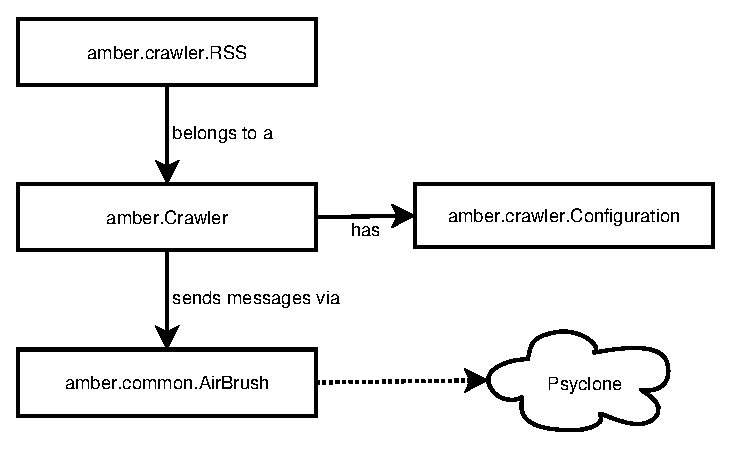
\includegraphics{image/crawler}
  \caption{
    Diagram of the design of the Crawler, the names are Java classnames, arrows
    mean that calls exist in the direction of the arrow.
  }
\end{figure}



\section{Objects in the amber.sieve package}

\classname{Configuration}

\begin{classmetadata}
\end{classmetadata}

\begin{interface}
\end{interface}



\classname{KeywordSpotter}

\begin{classmetadata}
  \implements{amber.common.AirBrushCallable}
\end{classmetadata}

\begin{interface}
\end{interface}



\section{Objects in the amber.showoff package}

\classname{Configuration}

\begin{classmetadata}
  \extends{amber.common.Configuration}
  \function{Store configuration}
\end{classmetadata}

\begin{interface}
  \method{void}{setValue}{String key}
    {Sets the value of key in the configuration.}
\end{interface}



\classname{EarthView}

\begin{classmetadata}
  \extends{java.awt.Canvas}
  \implements{Runnable}
\end{classmetadata}

\begin{interface}
  \init{EarthView}{}
    {Initializes the earthview display. It is a child of Canvas and can as such
    be used inside any application. Before starting the Earthview, first couple
    a Particle collection to it using setParticleCollection.}
  \method{\void}{setParticleCollection}{pc: Collection$\langle$Particle$\rangle$}
    {Sets the collection of particles to be displayed in the view.}
  \method{\void}{run}{}
    {Runs the thread (for Runnable).}
  \method{\void}{start}{}
    {Starts the thread, lets EarthView draw stuff.}
\end{interface}



\classname{FullScreen}

\begin{classmetadata}
  \extends{amber.ShowOffObject}
  \implements{amber.common.AirBrushCallable}
  % \function{}
\end{classmetadata}

\begin{interface}
  \init{FullScreen}{}
    {Initializes something.}
  \method{\void}{start}{}
    {Start the visualization.}
\end{interface}



\classname{Particle}

\begin{classmetadata}
  \function{Storage of particle data.}
  \data{An object of this class has information about its location and
    velocity, and it knows from which story it originates.}
\end{classmetadata}

\begin{interface}
  \init{Particle}{Story s}
    {Initializes a particle for Story s.}
  \method{\void}{launch}{}
    {Launches the particle, all parameters must be set, they cannot be changed
      afterwards.}
  \method{\void}{boost}{double}
    {Boost the particle in the direction it is heading. This can happen when
      for instance the Story gets replies or comments; boosting keeps the
      particle around longer.}
  \method{double}{getMass}{}
    {Gets the mass of the particle}
  \method{Vector$\langle$double$\rangle$}{getLocation}{}
    {Gets the location}
  \method{Vector$\langle$double$\rangle$}{getVelocity}{}
    {Gets the velocity}
  \method{Vector$\langle$double$\rangle$}{getAcceleration}{}
    {Gets the acceleration}
  \method{\void}{setMass}{double s}
    {Sets the mass of the particle to s}
  \method{\void}{setLocation}{Vector$\langle$double$\rangle$ v}
    {Sets the location to v}
  \method{\void}{setVelocity}{Vector$\langle$double$\rangle$ v}
    {Sets the velocity to v}
  \method{\void}{setAcceleration}{Vector$\langle$double$\rangle$ v}
    {Sets the acceleration to v}
  \method{\void}{setNewValuesAfter}{double t}
    {Calculates and sets new values using the current values after a period of
      time t}
\end{interface}



\classname{Applet}

\begin{classmetadata}
  \extends{java.applet.Applet}
\end{classmetadata}

\begin{interface}
\end{interface}



\begin{figure}
  \centering
  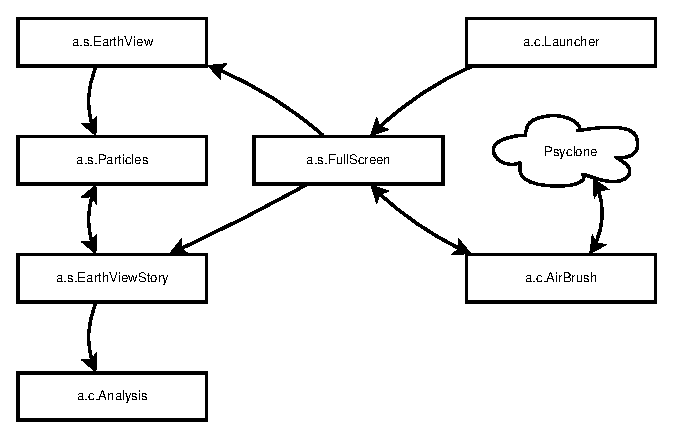
\includegraphics{image/showoff-fullscreen}
  \caption{
    Diagram of the design of the full screen ShowOff module, the names are
    abbreviated Java classnames
  }
\end{figure}





% \chapter{Conclusion}


% \appendix

\bibliographystyle{cadia}
\bibliography{bibliography}
\addcontentsline{toc}{chapter}{\refname}

\end{document}
